
\begin{center}
\textbf{Presenter:} \emph{Andrew Butterfield}
\end{center}

\section{Introduction}

At DASIA 2017\cite{Lero-DASIA17}
we discussed a modular approach to formally modelling
requirements, using a requirements baseline for a separation kernel developed
as part of the IMAKQP project\cite{IMAKQP-D02}.
This was based on work done using the CSP formalism\cite{hoare-1985:commuseque:},
done by two students for their dissertations \cite{KH-MCS2016,Costelloe17}.
Properties of interest could be explored and verified using
model-checking software such as FDR\cite{FDR3}.
That work followed on from recommendations we made for future work
in this area, including:
formalising the requirements baseline;
formalising kernel data-structure invariants;
and completing rough/draft CSP models explored during IMAKQP.

We consider that many useful formal modelling paradigms in this space
fall into two broad classes:
\begin{description}
  \item [State-Based]
    These are based on the notion of mutable state,
    usually organised as named variables, updated by assignment.
  \item [Process-Based]
    These communicate by message-passing, and persistent state
    is modelled as parameters to a process description.
    State change is captured by invoking the process with revised parameter values.
\end{description}
We shall illustrate these two paradigm classes by modelling a simple counter
system that supports two operations: counter initialisation, and count-up,
The count is observable, somehow.

A classic example of the state-based paradigm is
the Z specification language \cite{UsingZ}.
Here we consider the counter state as being stored
in a variable called $count$. Initialisation sets this variable to zero,
while counting up or down result respectively
in the variable being incremented or decremented.

In Z, which is a \emph{specification} language,
we model operations as relating their starting state (variable values)
to acceptable final states. Given variable \texttt{v},
we use the mathematical/logical variable $v$ to denote its starting value
before the operation commences,
and $v'$ to denote its value once the operation has completed.
In Z, a box-like graphical notation is used that has an operation name,
along with a declaration of its state observation variables,
follwed by predicates that describe the desired relationships that should hold.
\begin{schema}{CountInit}
  count,count' : \num
\where
  count' = 0
\end{schema}
\begin{schema}{CountUp}
  count,count' : \num
\where
  count' = count+1
\end{schema}
Z is very much aimed at specifying in a way
that suits ``standard'' impewative programming styles.

In the CSP formalism, we have (parameterised) processes
that participate in ``events'', and who subsequent behaviour
can depend on which event has just occurred.
We will imagine two events "init" and "up" that model respectively
the invocation of initialisation or counting-up.
We have a process called $Count$ that
is paramterised with a value we call $count$.
It's behaviour is that it performs
an ``external choice'' operation ($\extchoice$)
in which it offers to participate in either of the $init$ or $up$ events,
and then invokes itself recursively with a suitable revised parameter.
\begin{circus}
\circchannel init, up \\
Count(count) \circdef \\
\t1 init \then Circus(0) \\
\t1 \extchoice \\
\t1 up \then Count(count+1)
\end{circus}
The focus in CSP is on inter-process communication and concurrency.
This makes it very suitable for modelling requirements in a compositional
way, and is why it was initally chosen
as  a basis for modelling the IMAKQP baseline.
However, one problem with this approach is that the number of parameters
per process can get very large,
and state-changes that modify these are hard to scan and digest.

The work reported here explores a technique that aims to have the best of both
worlds, based on a formal paradigm known
as ``Unifying Theories of Programming'' (UTP) \cite{UTP-book}.
This uses 2nd-order classical predicate calculus,
where every predicate has an ``alphabet'' of variables that
model observations of a system that it is capable of describing.
The predicates relate before- and after-observations of a system,
using a similar convention that found in Z.

We do not go into details here, but show some standard UTP definitions
to give a flavour for how it works:

\begin{tabular}{ll}
\hline
   \textbf{Command} & \textbf{Semantics}
\\\hline
     $x:=e$
   & $x'=e \land v'=v$
\\   $P~;Q$
   & $\exists v_0 \bullet P[v_0/v'] \land Q [v_0/v]$
\\   $P\sqcap Q$
   & $P\lor Q$
\\   $P \lhd b \rhd Q$
   & $b \land P \lor \lnot b \land Q$
\\\hline
\end{tabular}

An alternative approach to just using Z, or CSP,
is taken by the language \Circus\cite{WC01,OCW2007},
which is a fusion of CSP with Z.
This allows individual named state components to be modified using simple
assignment statements, making descriptions easier to read.
It's formal semantics has been defined using UTP\cite{OCW2007}.


The \Circus\ language has been used to model requirements
for a haemodialysis machine\cite{DBLP:conf/asm/GomesB16},
in a similar way to how CSP was used to model kernel requirements.
This exploits the ability of \Circus\ to focus only on the relevant state changes.
However, as there is no model-checker for \Circus,
we have implemented an automated semantics-preserving translator to CSP
that allows FDR to be used for analysis.
In addition, there has been considerable work done by colleagues at
the University of York using the Isabelle/HOL theorem prover\cite{NPW02}
to encode the Unifying Theories of Programming (UTP) framework (\textsf{isabelle-utp}),
which is used as the basis for a formal semantics of \Circus,
and to build a series of useful proof automation techniques\cite{FosterZW14}.

This paper presents and discusses some investigations
into re-visiting the kernel requirements in \cite{IMAKQP-D02},
using \Circus\ as the modelling notation.
This provides the opportunity, in principle at least,
to use either model-checking or theorem-proving to perform analysis.

NEED MORE?
\section{Approaches}

An event is an abstraction of an observation of some change
or communication in a system. Events are considered atomic
(they happen completely, or not at all), and instantaneous.
An event can also have internal structure,
so it can be used to carry information over and beyond
just signalling that it has occurred.
The behaviour of system is defined in terms of:
(i) all the possible sequences of events that can be observed;
(ii) at each stage, what events are being blocked.
The state of a system captures which events it is willing to perform,
along with information about how its future behaviour depends on those events.
State can be represented implicitly by the ``call-graph'' structure of the model,
or, additionally,
some parts are given explicity as components whose values can change.

Typically, we build models with three key components,
each of which runs in parallel with the others,
synchronising on relevant events.
\begin{description}
  \item [Platform]
    An abstract model of how the platform (hardware/firmware) behaves,
    which is intended to model correct behaviour.
  \item [SUT]
   An abstract model of the software under test that interacts
   with the platform.
   This software can be either correct or incorrect depending on
   the analysis being performed.
  \item [Requirement]
   A model of the requirement under study, which basically monitors
   the software/platform interactions, keeping quiet as long as all is well,
   but forcing some kind of global error condition if it detects a violation.
\end{description}
A key principle here is to analyse each requirement independently,
to reduce the reasoning burden.
This is safe so long as each requirememt model is careful not
to constrain platform/software interactions.

The overall plan is to use the platform/requirement combination
to assess various models of the software behaviour,
both (hopefully) correct and faulty.
We want to run faulty software models through this approach verify that
the requirements cztch the relevant faults.
We want to run models of correct software, of increasing complexity,
in order to come up with (relatively) complete descriptions
of software behaviour, that can be used as formal specification
for high-level and low-level design stages, as well as code.


There are three basic approaches we can take
to modelling requirements using process-algebra notations:
event-based, parameter-based, and variable-based.

\paragraph{Event-based modelling} uses implicit state only,
with events modelling state-changes.
These events switch the behaviour of all three components above
to one that describes the behaviour associated with the new implicit state.
This was the approach used in the work reported at DASIA 2017 \cite{Lero-DASIA17}.

\paragraph{Parameter-based modelling}
uses read-only parameters in the definition of processes,
much like calling a function.
These encode various state parameters,
and there are conditional constructs that can be used to ensure
that subsequent behaviour is state-dependant.
This approach was used in a study in 2009
regarding Flash Memory devices\cite{DBLP:conf/sbmf/ButterfieldC09}.

\paragraph{Variable-based modelling} uses named global variables
to represent state components,
and assignment statements to update individual parts of that state.
In CSP, the only way to model these variables is as small processes
that support ``set'' and ``get'' events.
In \Circus, there is direct support for variables and assignment.
This approach was used in the haemodialysis study\cite{DBLP:conf/asm/GomesB16}.


\section{Tools}

The \Circus\ language has a concrete syntax based on \LaTeX,
and we have developed a parser for this, written in Haskell.
At present there are no suitable model-checkers
that work with \Circus\ directly,
but a deliverable from the H2020 INTO-CPS project\cite{compassd241}
gives a formal definition
of a translation from \Circus\ to CSP,
in order to facilitate the use of CSP model-checkers,
such as FDR\cite{FDR3} or PAT\cite{SunLDP09}.
We have mechanised that translation in Haskell,
targeting the CSP dialect used by FDR.

In addition we have two connections into
the Isabelle/HOL theorem prover:
\begin{enumerate}
  \item
    Using the \textsf{haskabelle} package,part of the standard distribution,
    allows our Haskell code to be translated into Isabelle/HOL,
    which facilitates its formal verification.
  \item
    An encoding of
    the Unifying Theories of Programming framework (UTP)
    called \textsf{isabelle-utp} has been developed
    at the University of York\cite{FosterZW14},
    which contains, among other things, formal UTP semantics for both CSP and
    \Circus.
    We can translate our \Circus\ and CSP abstract syntaxes into
    \textsf{isabelle-utp} notation,
    which allows us to use the theorem prover to check for desired properties.
\end{enumerate}

\subsection{Example}

One of the the requirements (PK-230) is that whenever partition code is running,
the processor must be in user mode.
In an abstract view,
the state of the system includes information about
what code is running (kernel/partition)
and the current processor privilege mode (user/supervisor).
A model of this requirement will simply track any changes
to those state components,
and raise an alert if it ever sees a (partition,supervisor) combination.

An abstract model of this for the platform
has four states with transitions triggered
by changes to whose code is running, and the processor privilege mode.
It can be visualised as the following state transition system,
where transitions $user$ and $super$ correspond to setting the privilege mode
and $krnl$ and $part$ denote switching to code belonging to the kernel or
a partition, respectively.

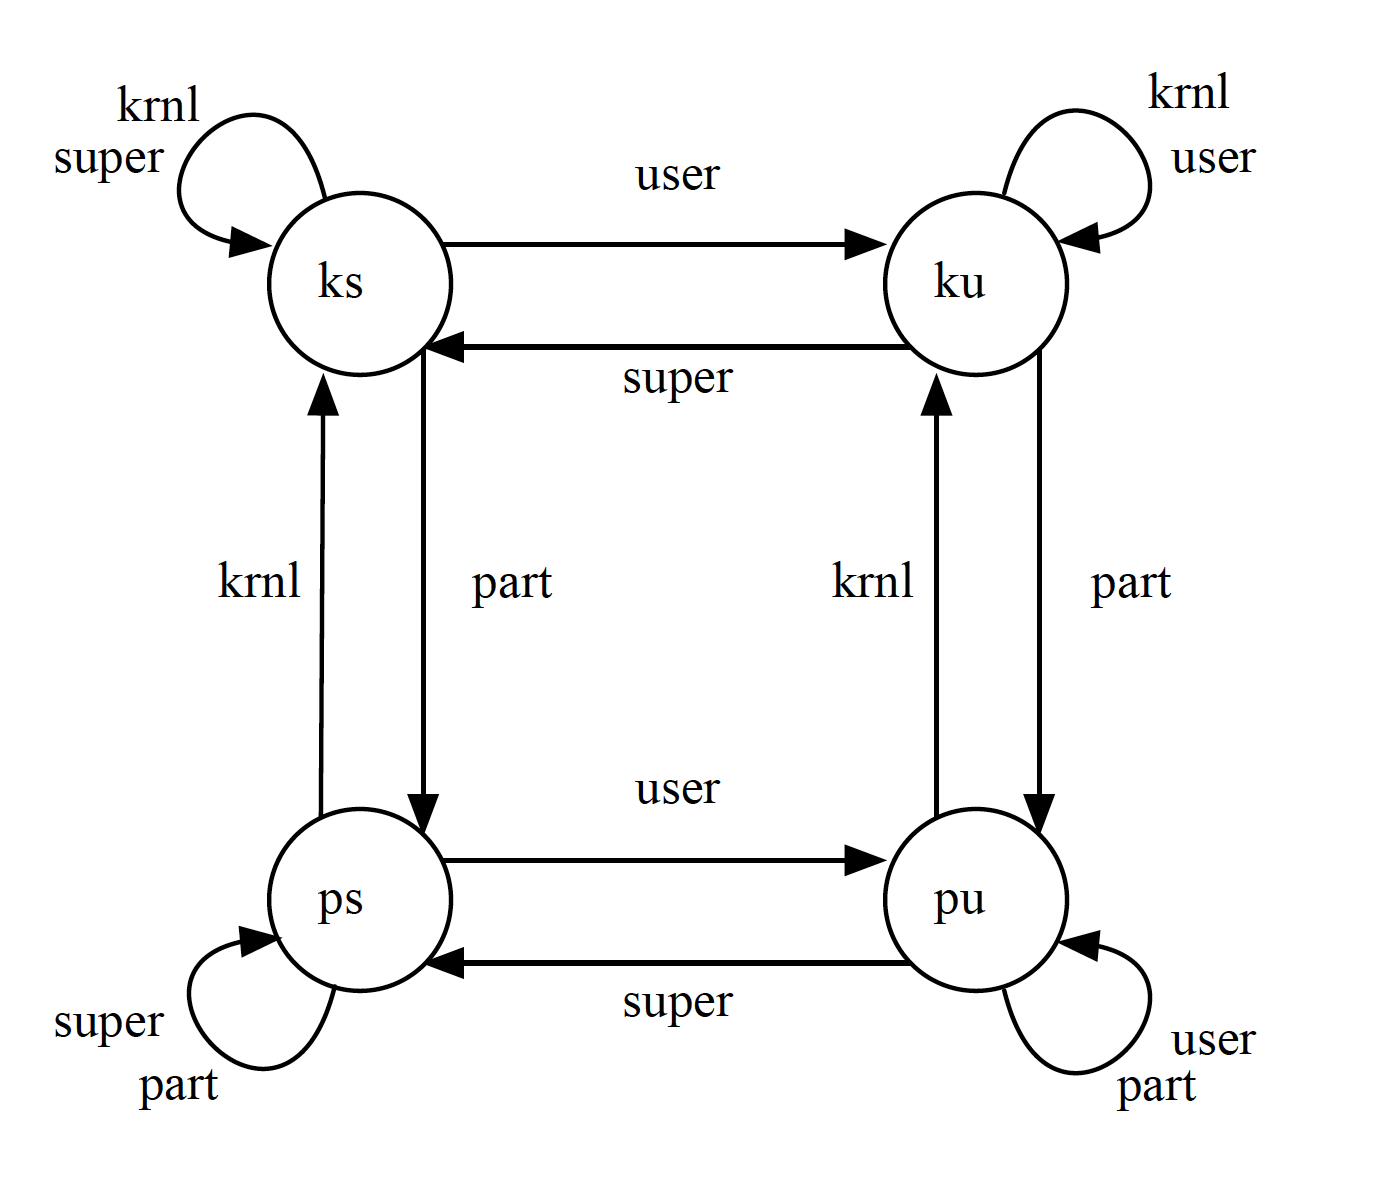
\includegraphics[scale=0.35]{images/CodeModelLTS}

The behaviour of the requirement PK-230 is to play along,
unless the system enters state $ps$
(\textbf{p}artition code running in \textbf{s}upervisor mode).
In this case it makes a $pk203fail$ transition, and then deadlocks.

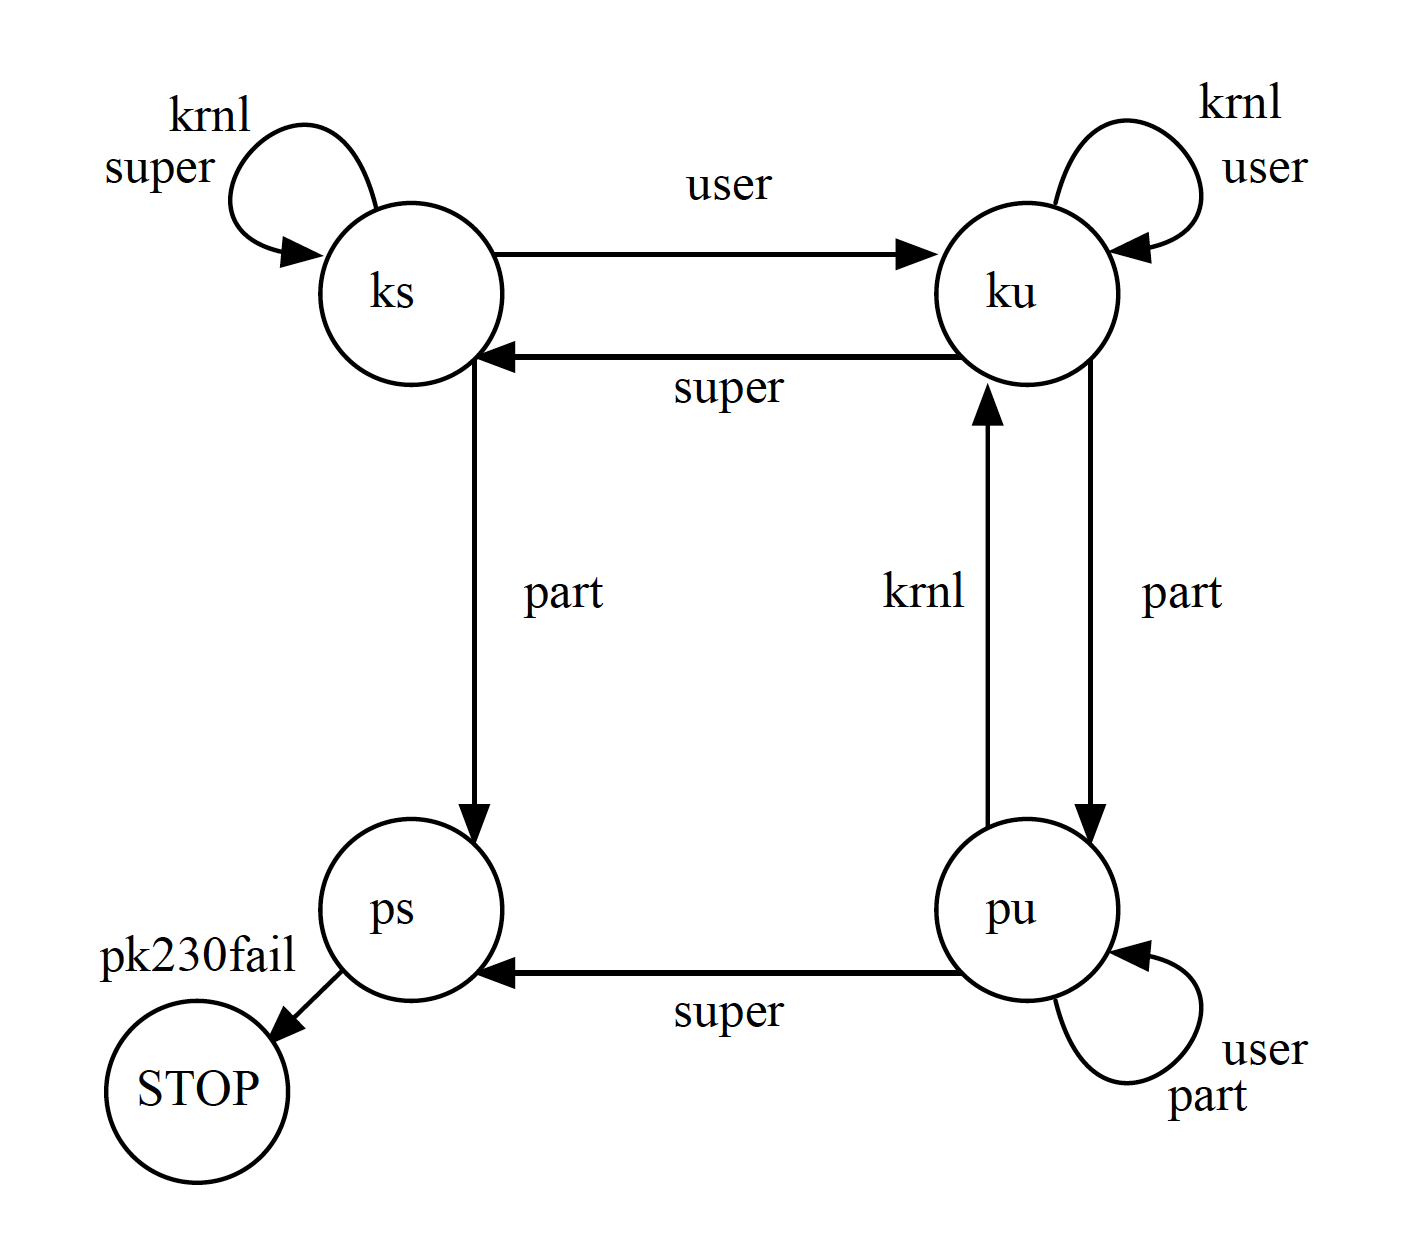
\includegraphics[scale=0.35]{images/PK230LTS}

We put these two in parallel, along with similar models for partition
and kernel code, all forced to agree on all transitions (except $pk230fail$).
If the kernel code model violates PK-230, then this combined model
will deadlock when it does.
This potential to deadlock can then easily be checked by a model-checker
such as FDR.
This basic idea, with different collections of states and transitions,
can be used to model most of the separation kernel requirements.
The challenge is to minimise the diversity of state and transitions,
by sharing them among as many requirements as possible.

The ultimate goal is that such modelling would lead to comprehensive models
of correct kernel code,
which could them form the basis for formal specifications of that code.
These could then be used as a kick-off point to formally verify selected
portions of said code.

% \paragraph{Event-based example}
% uses events $swk$, $swp$ (switch to kernel/partition)
% and $usr$, $sup$ (set user/supervisor mode) and a requirement process
% whose monitoring criteria changes based on the most recent switch event.
% \begin{circus}
% PK230k ~\defs~ e:\{swk,usr,sup\} \then PK230k
% \\ \qquad \qquad \quad {} \extchoice swp \then PK230p
% \\
% PK230p ~\defs~ e:\{swp,usr\} \then PK230p
% \\ \qquad \qquad \quad {} \extchoice swk \then PK230k
% \\ \qquad \qquad \quad {} \extchoice sup \then pk230fail \then Stop
% \end{circus}


\section{Investigation}

We are conducting an on-going investigation into how to formalise
the separation kernel requirements in \cite{IMAKQP-D02},
with an ultimate view to providing a basis for the formal verification
of selected parts of kernel sources w.r.t. those requirements that
may be difficult to test adequately.
Using the \Circus\ notation we are exploring modelling approaches
such as those described above
to assess them in terms of clarity, ease of model-checking, proof support,
and their utility in deriving formal specifications of code behaviour.
This talk and paper will describe progress to date.
